\section{Taxonomy and Benchmark Coverage}
\label{sec:taxonomy}

The benchmark becomes readable once it is organized as two taxonomies. The first taxonomy is algorithmic: loop-based, window-based, model-based, adaptive, and data-driven estimators all occupy distinct parts of the design space. The second taxonomy is physical: clean standards-style ramps, steps, and modulation tests live beside IBR-specific harmonics, ringdowns, and composite multi-event stress. The benchmark is not large for its own sake; it is large because those axes interact.

\begin{figure}[t]
\centering
\resizebox{\columnwidth}{!}{%
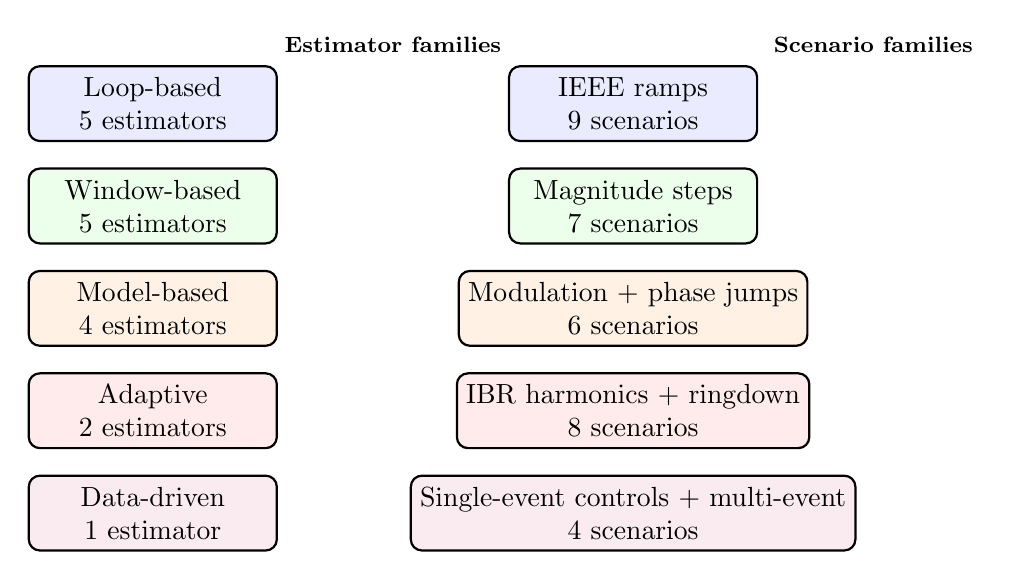
\begin{tikzpicture}[
  fam/.style={draw, rounded corners, thick, align=center, minimum width=3.15cm, minimum height=0.95cm, fill=gray!10},
  small/.style={font=\footnotesize}
]
\node[fam, fill=blue!8] (e1) at (0, 3.6) {Loop-based\\5 estimators};
\node[fam, fill=green!8] (e2) at (0, 2.3) {Window-based\\5 estimators};
\node[fam, fill=orange!10] (e3) at (0, 1.0) {Model-based\\4 estimators};
\node[fam, fill=red!8] (e4) at (0, -0.3) {Adaptive\\2 estimators};
\node[fam, fill=purple!8] (e5) at (0, -1.6) {Data-driven\\1 estimator};

\node[fam, fill=blue!8] (s1) at (6.1, 3.6) {IEEE ramps\\9 scenarios};
\node[fam, fill=green!8] (s2) at (6.1, 2.3) {Magnitude steps\\7 scenarios};
\node[fam, fill=orange!10] (s3) at (6.1, 1.0) {Modulation + phase jumps\\6 scenarios};
\node[fam, fill=red!8] (s4) at (6.1, -0.3) {IBR harmonics + ringdown\\8 scenarios};
\node[fam, fill=purple!8] (s5) at (6.1, -1.6) {Single-event controls + multi-event\\4 scenarios};

\node[small] at (3.05, 4.35) {\textbf{Estimator families}};
\node[small] at (9.15, 4.35) {\textbf{Scenario families}};
\end{tikzpicture}
}
\caption{Two complementary taxonomies organize the benchmark. The left side describes algorithmic assumptions; the right side describes disturbance families. Their interaction, not any single axis alone, drives the benchmark conclusions.}
\label{fig:taxonomy_map}
\end{figure}

The estimator taxonomy explains why a flat ranking is unstable. Loop-based methods are cheap and attractive for embedded deployment, but they can become fragile under large phase discontinuities. Window-based methods often look better on trip-risk or spectral pollution but pay window latency and compute. Model-based filters occupy a middle-cost regime with strong average accuracy when the state model is informative. Adaptive methods are lightweight but less robust in the hardest cases. The single data-driven method in the benchmark, Koopman (RK-DPMU), is best read as a reduced-order alternative rather than as a universal neural surrogate.

The scenario taxonomy is equally important. The clean standard families mostly separate estimators by accuracy because many methods already tie at zero trip-risk. The IBR families are different: harmonic stress, noisy ringdown, and especially the composite multi-event case create disagreements between RMSE, peak error, and trip-risk leaders. That is why the full scenario catalog appears in the appendix rather than being collapsed into a one-line ``dataset'' description.

\begin{figure*}[t]
  \centering
  
\includegraphics[width=0.98\textwidth,height=0.48\textheight,keepaspectratio]{Fig1_Scenarios_Final.pdf}
  \caption{Representative benchmark scenarios from the study. The figure mixes clean standard events with composite IBR stress, illustrating why the benchmark must be read by disturbance family rather than through a single aggregate score.}
  \label{fig:scenario_overview}
\end{figure*}

Figure~\ref{fig:scenario_overview} makes the reporting problem visible. A clean magnitude step and a composite IBR multi-event sequence should not be expected to produce the same ranking, even if both are called ``frequency estimation'' tests. The manuscript therefore treats scenario family as part of the experimental design, not as decoration around a final leaderboard. Full estimator and scenario catalogs are provided in Appendices~\ref{app:estimators} and~\ref{app:scenarios}.
